\providecommand{\home}{../../..}
\documentclass[\home/main.tex]{subfiles}
\usetikzlibrary[arrows,snakes,backgrounds]

\begin{document}

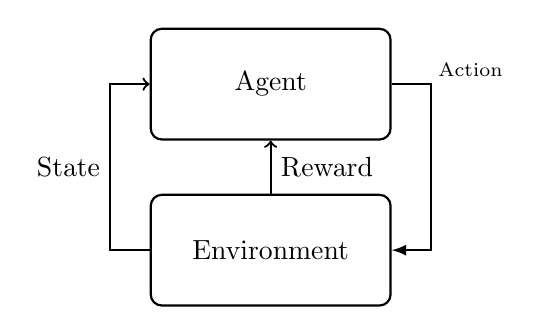
\begin{tikzpicture}[node distance = 6em, auto, thick]
    \tikzset{
        block/.style={
                rectangle, draw, text width=8em, text centered, rounded corners, minimum height=4em
            },
        connector/.style={
                -latex,
                font=\scriptsize
            },
        descr/.style={
                fill=white,
                inner sep=2.5pt
            },
        connector/.style={
                -latex,
                font=\scriptsize
            },
        rectangle connector/.style={
                connector,
                to path={(\tikztostart) -- ++(#1,0pt) \tikztonodes |- (\tikztotarget) },
                pos=0.5
            },
        rectangle connector/.default=-2cm,
        straight connector/.style={
                connector,
                to path=--(\tikztotarget) \tikztonodes
            }
    }

    \node[block]   (agent)                                           {Agent};
    \node[block]        (env)       [below of=agent]                      {Environment};

    \draw [->] (env) to node [auto, swap] {Reward} (agent);
    \draw [->] (env.west) -- ++(-0.5,0) |- node[pos=0.25] {State} (agent.west); % first go left a bit, then go vertical and horizontal to agent node while putting a label with name "State" on it
    % \draw [->] (agent.east) --++(0.5,0) |- node[pos=0.25] {Action} (env.east);
    \draw [rectangle connector=0.5cm] (agent.east) to node[descr,pos=2] {Action} (env.east);

\end{tikzpicture}
\end{document}
